\section[Design Strategy]{Design Strategy on Embedded (Real-time) Software}
\subsection{Targets}
\begin{itemize}
	\item Design should be solution independent for as long as it makes sense (not as long as possible).
	\item Encourage system design, rather than separate designs for mechanics, electronics, firmware, software, etc., which may be conflicting
	\item System specification is ideally done using a unique specification language, not in prose
	\item The specification can be simulated (executed)
	\item Implementations can be easily changed, e.g. from HW to SW or vice versa.
\end{itemize}

\subsection{Requirements for Practical Application}
\begin{itemize}
	\item Methods and tools should not be too technical in system design, i.e. methods should be applicable for electronics, firmware and if possible also mechanics developers
	\item If possible good tool support and automatic synthesis
\end{itemize}

\subsection{Specification Languages}
\begin{itemize}
	\item Formal languages are unique
	\item Examples of specification languages: SystemC, SysML, SpecC, SystemVerilog, Esterel, Matlab/Simulink, Statecharts.
	\item The specification can be compiled and executed
	\item Simulations of the system on a powerful system (e.g. PC) are mostly supported
	\item The executable specification serves as golden reference for future development steps
\end{itemize}

\subsection{Approach}
Approach in a real time embedded design for task and scheduling topics
\begin{enumerate}
	\item Analysis of requirements and split work up into tasks
	\item The system and task model
	\item The scheduling algorithm with related schedule ability test.
	      Implement every flow and measure WCET.
	\item Theoretical and/or empirical performance evaluation of the scheduling algorithm and/or the schedule ability test
\end{enumerate}

\subsubsection{Enhanced with Multicore}
Real-time scheduling analysis usually focuses on three components that build on one another:
\begin{enumerate}
	\item Define the work to be done
	\item The system and task model / Manually determine concurrency
	\item Software architecture considering the parallelism
	      \begin{enumerate}
		      \item Add some additional data required to make concurrency easier
		      \item Organize into an algorithm
		      \item Determine the partitioning
		      \item Determine the communication model
		      \item Map the processing to the cores of the processor
	      \end{enumerate}
	\item The scheduling algorithm with related schedule ability test. Implement every flow and measure WCET.
	\item Theoretical and/or empirical performance evaluation of the scheduling algorithm and/or the schedule ability test
\end{enumerate}

\subsubsection{Split Work up into Tasks}
Get the system's timing constraints from \ldots
\begin{itemize}[label=\ldots]
	\item the physics of the system and their implications
	\item the application
\end{itemize}
Data flow charts help to split ub data paths into tasks.

\subsubsection{Classify Tasks}
\begin{minipage}[b]{0.6\textwidth}
	First task of a system architect is to classify the tasks into the structure like below.
	Every task of a lower class can be implemented in a higher class.
	A task without timing constraints mostly does not exist, however for the sake of completness it is arranged and shown here.
	Strict periodic and event driven tasks are similar in their priority since they are both implemented in ISR.
\end{minipage}
\begin{minipage}{0.39\textwidth}
	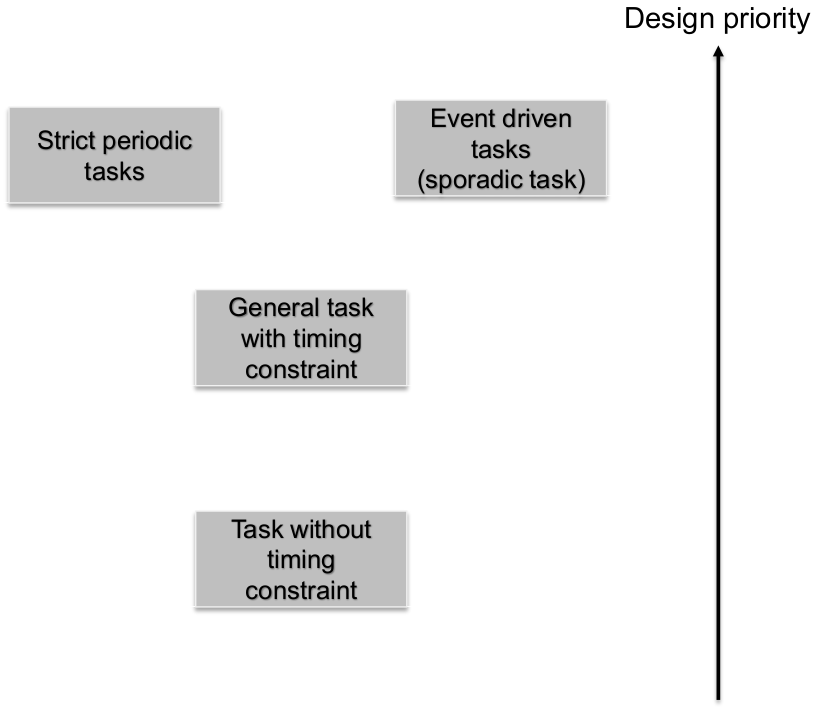
\includegraphics[width=\textwidth]{images/DesignStrategy/classify_tasks.png}
\end{minipage}


\subsubsection{Implementation without RTOS}
% \begin{minipage}[b]{0.6\textwidth}
The classification leads to the implementation in three different areas: Timer-ISR, ISR and main.
First steps can and should be implemented and tested separately.
Especially to determine WCET.
Since the ISR influence each other, tests must be undertaken with both implementations.
Last Step is to test the whole software architecture concerning real time behavior.

% \end{minipage}
% \begin{minipage}{0.39\textwidth}
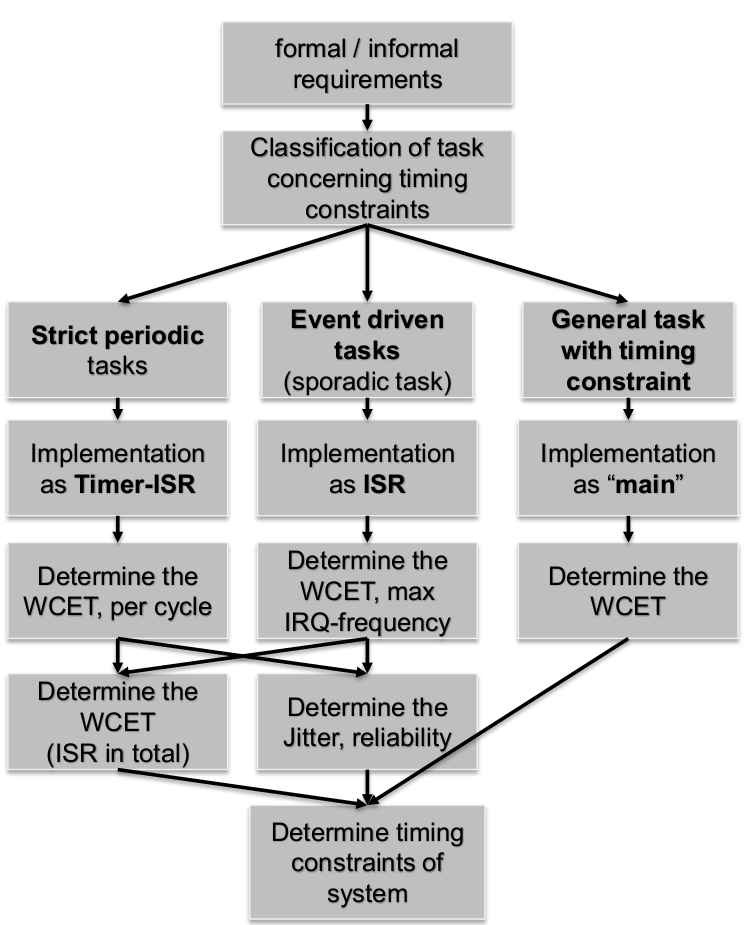
\includegraphics[width=0.4\textwidth]{images/DesignStrategy/task_implement_no_rtos.png}
% \end{minipage}

\subsubsection{Implementation with RTOS}
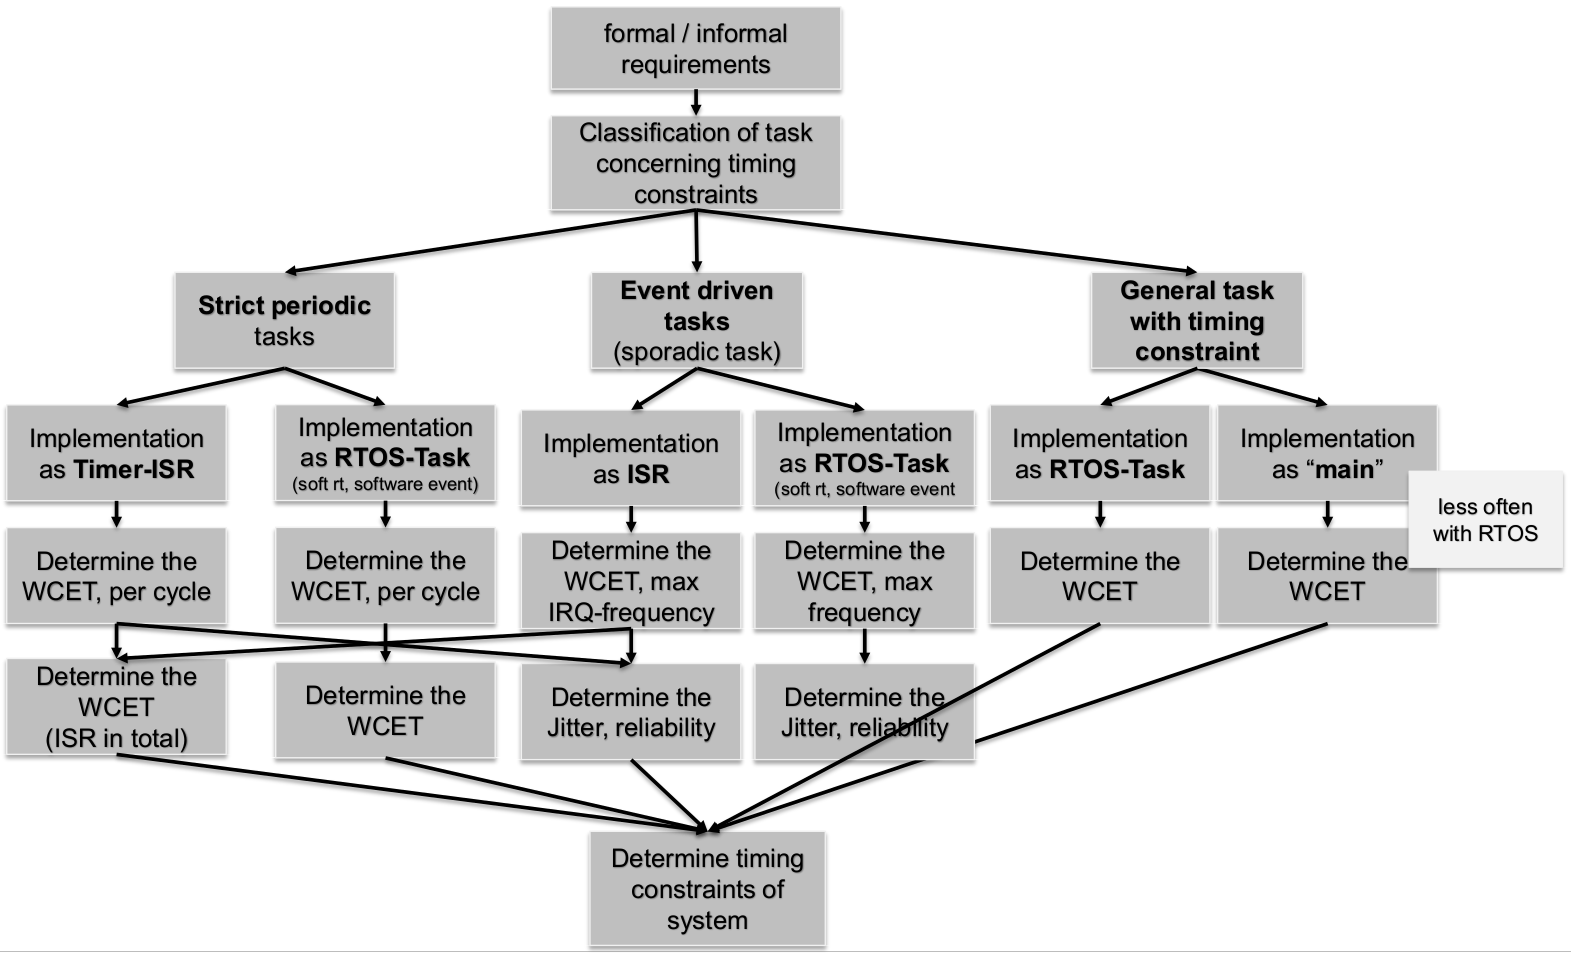
\includegraphics[width=0.9\textwidth]{images/DesignStrategy/task_implement_rtos.png}

\subsection{Approaches to define static Priorities for Tasks}
\subsubsection{Rate-Monotonic Approach: Short Code High priority}
The idea is that short ISR/tasks are executed fast.
Therefore, they block fo a very short time and execution is more guaranteed by priority.
\begin{itemize}
	\item Shortest ISR has highest priority
	\item Shortest flow/task has highest priority
\end{itemize}

\subsubsection{Important Code High Priority}
The idea is important ISR/tasks are executed fast.
\begin{itemize}
	\item Important ISR has highest priority
	\item Important task has highest priority
\end{itemize}

\subsubsection{Blended Approach}
Combination of RMA and ICH
\begin{itemize}
	\item Short task high priority
	\item Important ISR has high priority
\end{itemize}

\subsection{Interrupt Handling Concepts}
There are two main concepts how interrupt handling is implemented.

\begin{table}[h]
	\begin{tabularx}{\textwidth}{lXX}\hline
		Name        & Service Routine (ISR)                            & RTOS Task                                          \\\hline
		Description & Event code is executed mainly in the ISR         & ISR passes every executing code to RTOS task       \\
		Pros        & - Fastest execution                              & - RTOS support\newline - Interrupts fast available \\
		Cons        & - No or small RTOS support\newline - Blocks RTOS & - Slower execution, depended on RTOS scheduling    \\\hline
	\end{tabularx}
\end{table}

The approach of: \textbf{Interrupt handler in the RTOS task} is also called \textbf{software events} approach.
In a project they can also be combined.

\subsection{Prioritizing Interrupts, RTOS and Handling}
The real time system architecture can be influenced by defining the priority of the system timer of the RTOS!
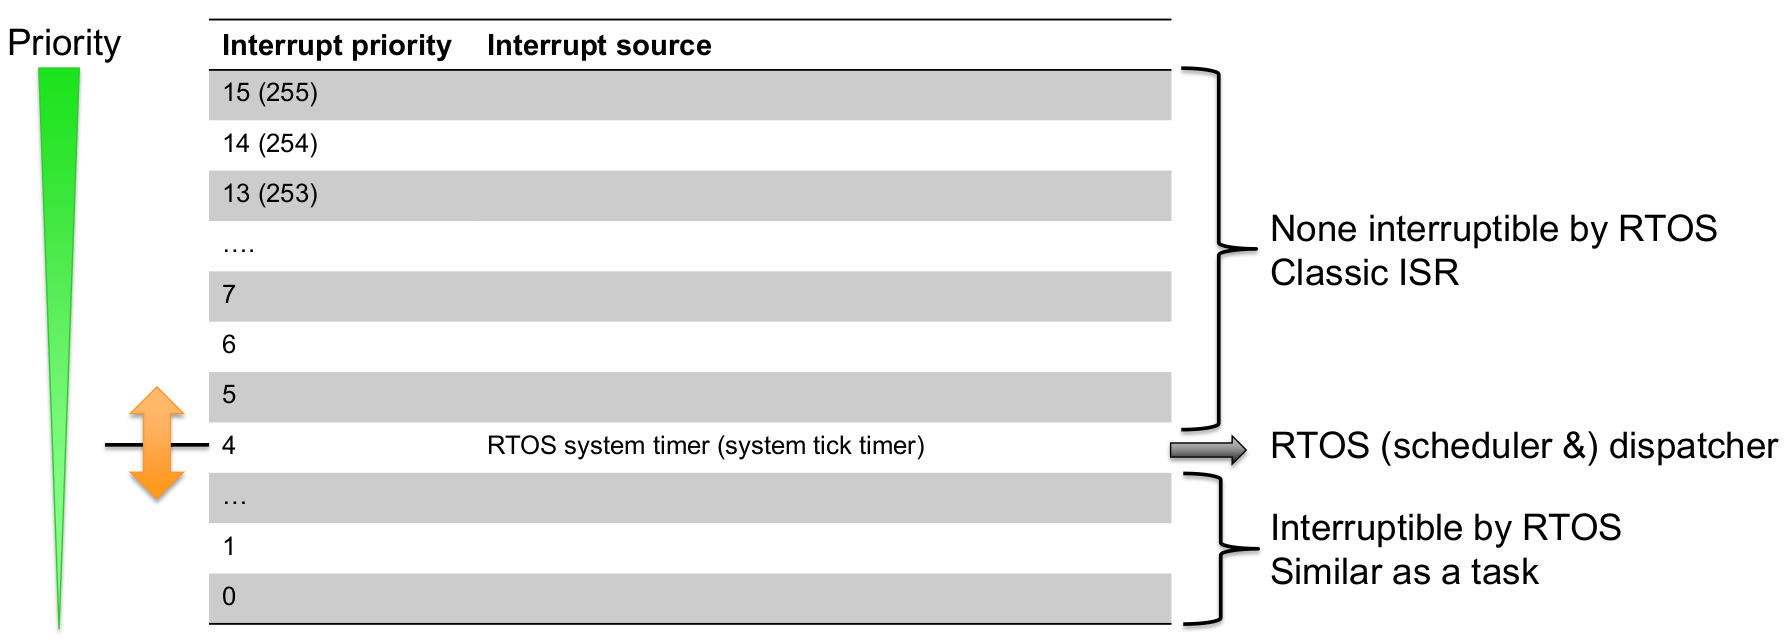
\includegraphics[width=\textwidth]{images/DesignStrategy/prio_interrupts.png}
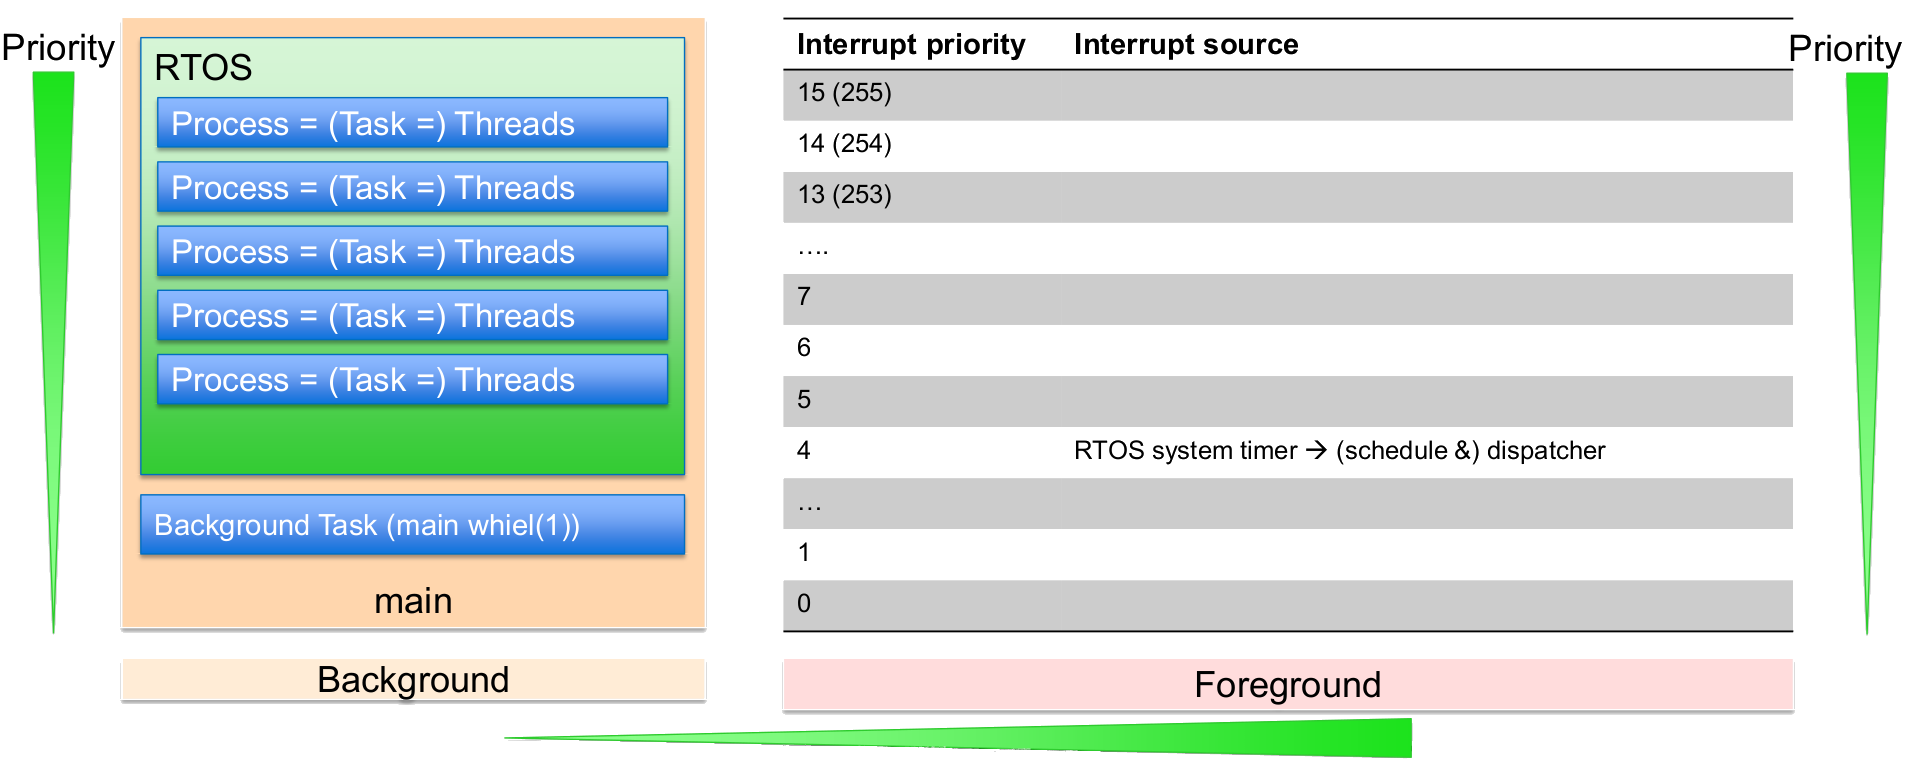
\includegraphics[width=\textwidth]{images/DesignStrategy/prio_interrupts_rtos_handling.png}
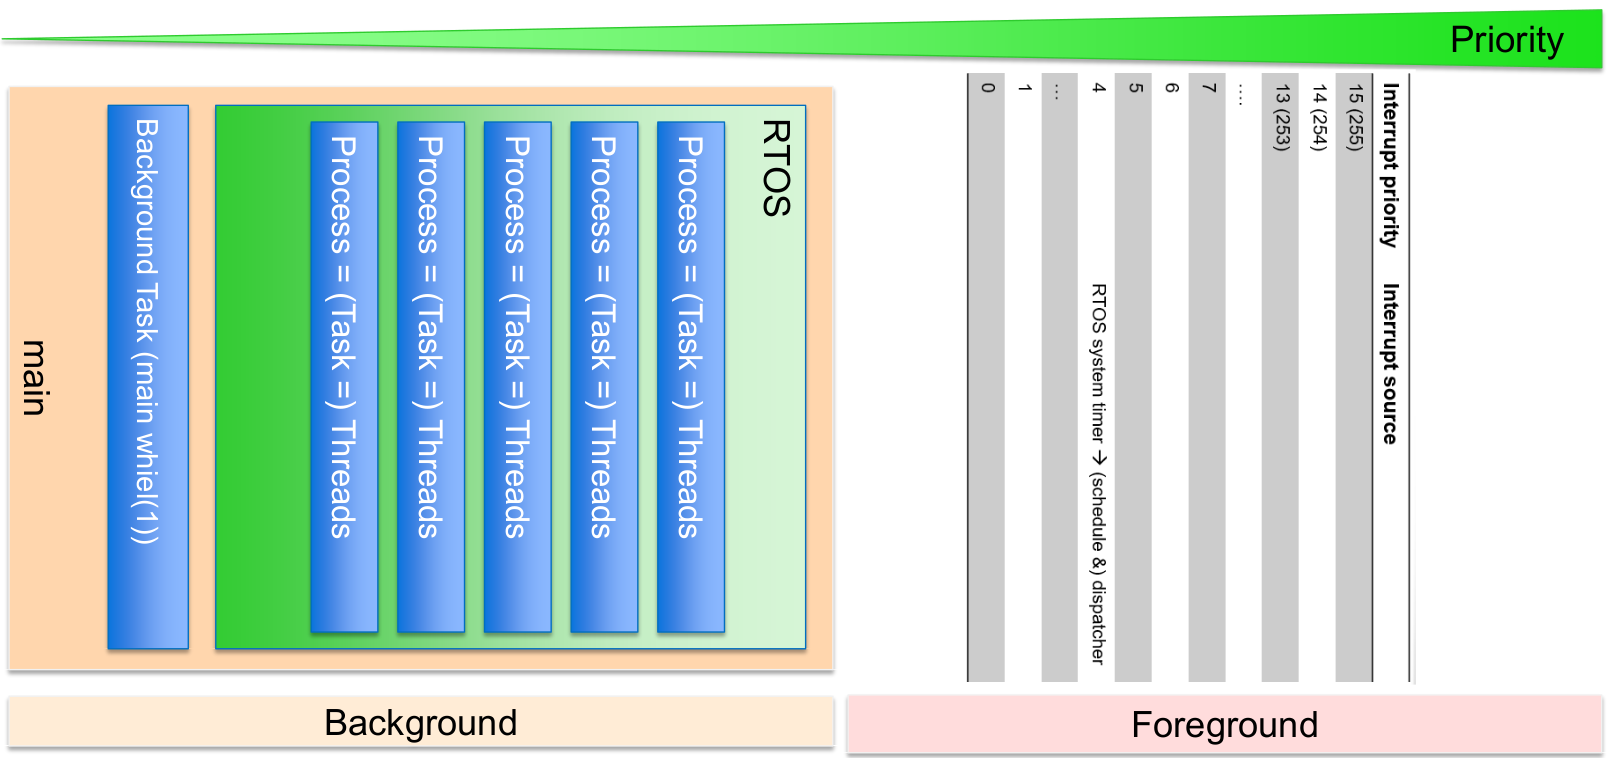
\includegraphics[width=\textwidth]{images/DesignStrategy/prio_interrupts_rtos_background.png}

\subsection{Assessment}
During the design approach the folowing assessment can be done accordingly to the following slides.
However, the following process should e cared out in phase 1, 2 and 3!
\begin{description}
	\item[Jitter Time] The temporal jitter $T_\text{jitter}$ specifies the time with which the start of the reaction routine is allowed to fluctuate.
	      Reasons for this can be time-synchronous activities, for which only small deviations are acceptable.
	      If the acceptable jitter time is below approx. 100 instruction execution times, it can be assumed with certainty that the requirement is in a critical range for processors.
	      The uncritical limit above which the processor can be expected to behave in a guaranteed manner can be expected, is of course individually dependent on the system.
	      In any case, the system is designed to be safe if the permitted jitter is greater than the sum of all higher-priority events (taking into account the frequency of occurrence).
	      For event-controlled systems if the jitter is greater than the sum of the cycle time for time-controlled systems
	\item[Service Time] The service time $T_\text{service}$ plays a seemingly unimportant role, since it has to be scheduled anyway.
	      However, for service times that take up more than 30\% of the total time (in the normal case or worst case), one must assume that this time is very dominant and strongly influences the other parts of the
	      systems strongly. However, this 30\% limit is fuzzy, while service times < 1\% certainly have no influence.
	\item[Reaction Time (WCET)] The maximum required reaction time $T_\text{reaction}$ is made up of the latency time and the service time.
	      However possible interruptions must also be considered and taken into account.
	      It becomes critical for the reaction time when it is about < 100 Instruction cycles (the limit is again	individual).
	      The uncritical limit is again reached at the sum of all reaction times or the cycle time.
\end{description}

\subsubsection{Interaction of the Criteria}
Even if the Reaction Time is the sum of Jitter and Service time the single criterie mus also be met to get a feasable embedded real time system. See table \ref{tab:crit_times}.

Adjusting screws on the system:
Requirements, chosen System, CPU frequency $\rightarrow$ instruction cycles, Ssoftware design $\rightarrow$ $T_{service}$\%

\begin{table}[h]
	\caption{Criteria for uncritial/critical timings}
	\label{tab:crit_times}
	\begin{tabularx}{\textwidth}{l X X}\hline
		Requirement         & Rate as Critical                     & Rate as Uncritical                                                                                      \\\hline
		$T_\text{jitter}$   & $< 100\times$ instruction cycles     & > Sum of all higher prioritised reaction times\newline OR\newline > Cycle time (time-controlled system) \\
		$T_\text{service}$  & $> 30\%$ of the total computing time & $<1\%$ of the total computing time                                                                      \\
		$T_\text{reaction}$ & $< 100\times$ instruction cycles     & > Sum of all higher prioritised reaction times\newline OR\newline > Cycle time (time-controlled system) \\\hline
	\end{tabularx}
\end{table}

\paragraph{Example for 100\;MHz Instruction Time}
For this example a microcontroller with 100\;MHz RISC architecture is assumed.
(consequently every 10ns (0.00001ms) an instruction is executed).
The Boundary is therefore 0.001ms.
A Simple Model would use constant latency times.
More complex would it be with variable latency depending on system complexity.
The Microcontroller can achieve faster reaction time when the task is implemented purely in ISR.
This diagram is not sharp and must be interpreted according to the system and project requirements.
But it gives a impression.

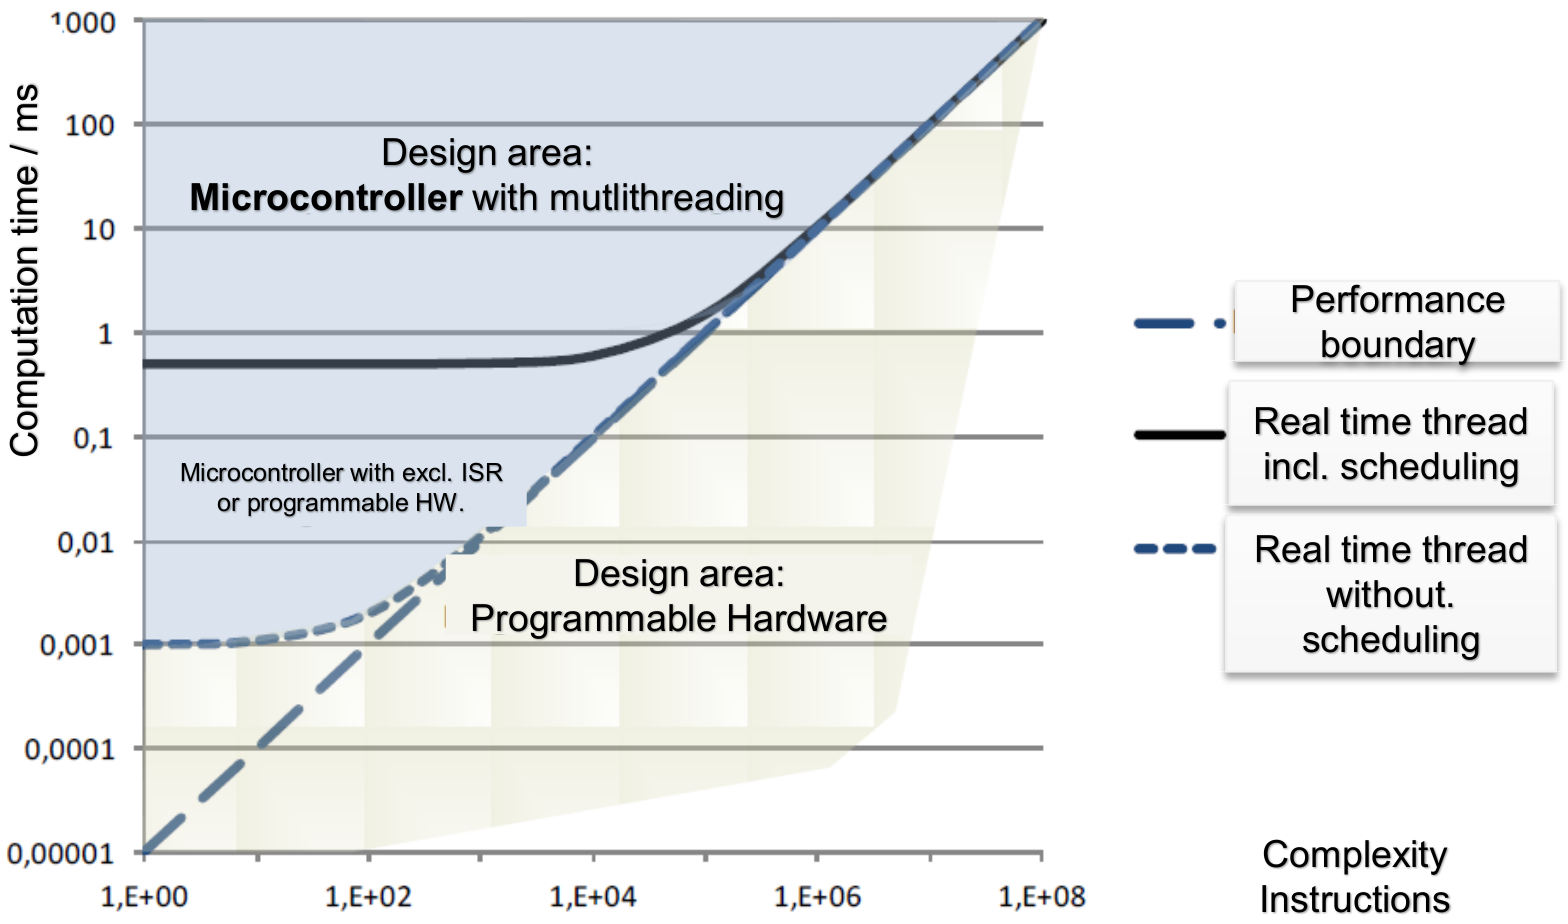
\includegraphics[width=0.8\textwidth]{images/DesignStrategy/100mhz_example.png}

The decision tree is true for the 100\;MHz example.
It gives a specific idea where the limitations of an embedded real time system, based on MCUs, lie.
Depending on the system there can be more sophisticated solutions possible.

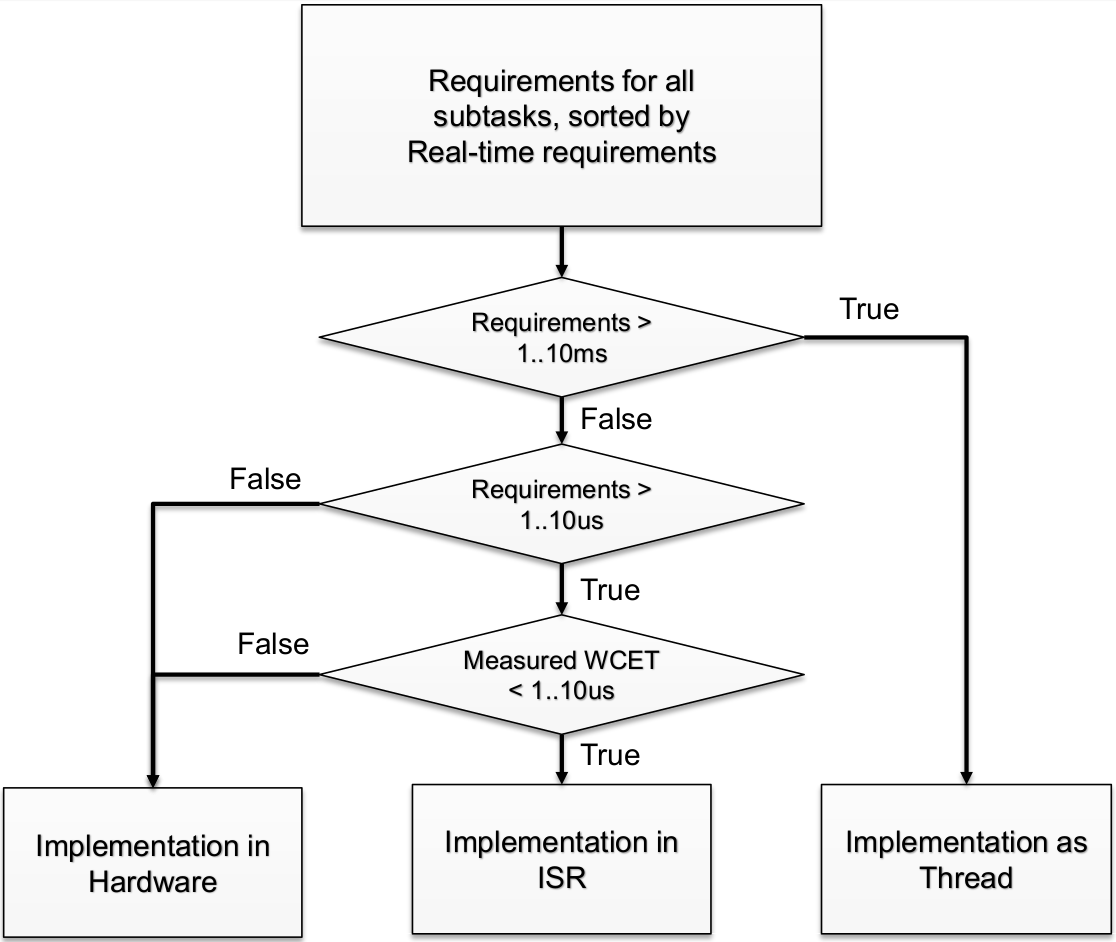
\includegraphics[width=0.6\textwidth]{images/DesignStrategy/decision_tree.png}